\documentclass[spanish,notes=hide]{beamer}

%Para crear una versión 'handout' (Copyright: Diego Berrueta)
%\documentclass[handout,notes=show]{beamer}

\usetheme{Warsaw}
\usepackage{beamerthemesplit}

\usepackage[spanish]{babel}
\usepackage[utf8]{inputenc}
\usepackage{listings}
\usepackage{graphicx}
\usepackage{colortbl}

\title{SWAML}
\subtitle{Publicaci\'on de listas de correo en Web Sem\'antica}
\author{Sergio Fern\'andez L\'opez}
\institute{%
	\href{http://swaml.berlios.de/}{http://swaml.berlios.de/}\\
	\vspace{0.7cm}
	Proyecto Fin de Carrera\\
	E.U. de Ingenier\'ia T\'ecnica en Inform\'atica de Oviedo
}
\date{20 de Diciembre de 2006}

\begin{document}

\frame{
  \note[item]{Saludar}
  \note[item]{Presentarse}
  \note[item]{Con su permiso procederé a presentarles mi proyecto fin de carrera 
    \textit{SWAML, publicación de listas de correo en Web Semántica}}

  \titlepage
}

%\frame{\tableofcontents}

\section{Introducción}

\subsection{Situación actual}
\frame
{
  \frametitle{Panorama actual}

  \note[item] {	Miles de listas de correo de las más variopinta temática }
  \note[item] {	Publicación en HTML de los archivos antiguos }
  \note[item] {	Pérdida de toda posibilidad de recuperar esa información }
  \note[item] {	Marcado estructurado sin valor semántico (problemas de internacionalización 
		y accesibilidad entre otros) }
  \note[item] {	Duplicidad de datos para los motores de búsqueda tradicionales }

  \begin{itemize}
   \item<2-> \textbf{Situación:}
	\begin{itemize}
	  \item Miles de listas de correo
	  \item Publicación en HTML
	\end{itemize}
   \item<3-> \textbf{Problemas:}
	\begin{itemize}
	  \item Pérdida de información
	  \item Marcado estructurado sin valor semántico
	  \item Problemas en las búsquedas tradicionales
	\end{itemize}
  \end{itemize}
}
\frame
{
  \begin{center}
	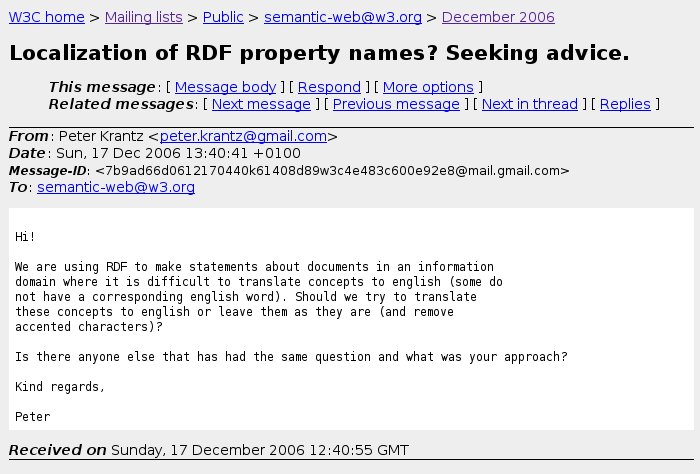
\includegraphics[width=0.9\textwidth]{images/lista-html.png}
  \end{center}
}

\subsection{Objetivos}
\frame
{
  \frametitle{Objetivos}
  FIXME: no me gusta
  \begin{itemize}
   \item<1-> Objetivo principal: 
     \begin{itemize}
      \item \textbf{Publicación de los archivos antiguos de listas de correo en un formato rico semánticamente.}
     \end{itemize}
   \item<2-> Varios objetivos secundarios:
	\begin{itemize}
	  \item Maximizar la reutilización de la infraestructura disponible previamente.
	  \item Desarrollar un prototipo capar de recomponer listas de correo \textit{atacando} 
		colecciones de ficheros RDF.
	  \item Abrir la puerta a nuevas aplicaciones.
     	\end{itemize}
  \end{itemize}
}
\frame
{
\frametitle{mbox}
FIXME:listings
\begin{center}
%\begin{verbatim}
...
From sioc-dev@googlegroups.com Fri Sep 15 13:35:44 2006
Message-ID: <1158352519.450b0e871c79e@courrier.privatedns.com>
Date: Fri, 15 Sep 2006 16:35:19 -0400
From: Frederick Giasson <fred@fgiasson.com>
To: sioc-dev@googlegroups.com
Subject: Implementation of the SIOC v1.08 ontology in Talk Digger
...
From sioc-dev@googlegroups.com Tue Sep 19 07:10:22 2006
From: Kjetil Kjernsmo <kjetilk@opera.com>
Organization: Opera Software ASA
To: sioc-dev@googlegroups.com
Subject: Re: User vs. Person complexity
Date: Tue, 19 Sep 2006 16:09:15 +0200
...
%\end{verbatim}
\end{center}
}

\subsection{La Web Semántica}
\frame
{
  \frametitle{Introducción a la Web Semántica (I)}

  \begin{itemize}
   \item<1-> Tim Berners-Lee expuso en 2001 su visión de lo que sería la Web Semántica:
     \begin{quote}
	\emph{«... \textbf{disponer datos} en la Web \textbf{definidos y enlazados} 
	de forma que puedan ser \textbf{utilizados por las máquinas}, no solamente 
	para visualizarnos, sino también para \textbf{automatizar} tareas, 
	\textbf{integrar} y \textbf{reutilizar} datos entre aplicaciones.»}
     \end{quote}
   \item<2-> En definitiva, \begin{Large}\textbf{una web más útil}\end{Large}.
  \end{itemize}
}
\frame
{
  \frametitle{Introducción a la Web Semántica (II)}

  \begin{columns}
    \begin{column}{0.6\textwidth}
	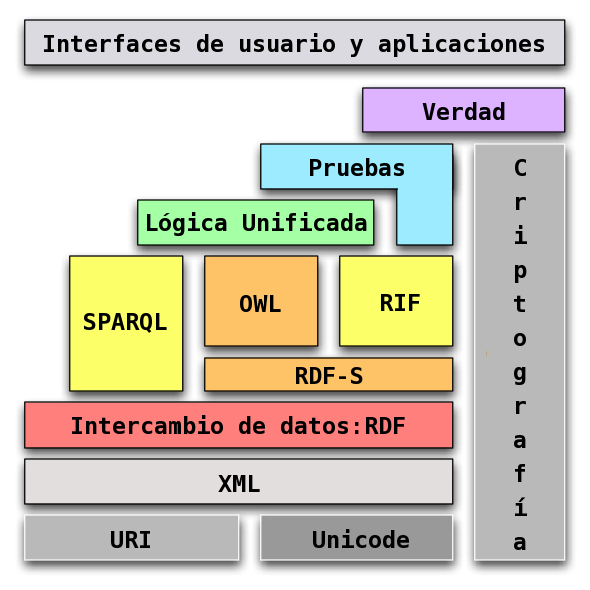
\includegraphics[width=\textwidth]{images/pila-web-semantica.png}
    \end{column}
    \begin{column}{0.4\textwidth}
      Tecnologías:
      \begin{itemize}
	\item \textbf{RDF} (\textit{Resource Description Framework})
	\item \textbf{OWL} (\textit{Web Ontology Language})
	\item \textbf{SPARQL} (\textit{SPARQL Protocol and RDF Query Language})
      \end{itemize}
    \end{column}
  \end{columns}
}
\frame
{
  \frametitle{RDF}

  \note[item]{	RDF se basa en un modelo de tripletas. El sujeto es un recurso, identificado
		por una URI, que se relaciona mediante un predicado binario con el objeto, que 
		puede ser otra URI o un literal.}
  \note[item]{	Cada tripleta puede verse como un arco, y al juntarse con otros arcos 
		se obtiene un grafo dirigido que describe los recursos y las relaciones 
		entre todos los recursos.}

  \begin{center}
    Modelo de tripletas del tipo \texttt{(sujeto, predicado, objeto)}:
    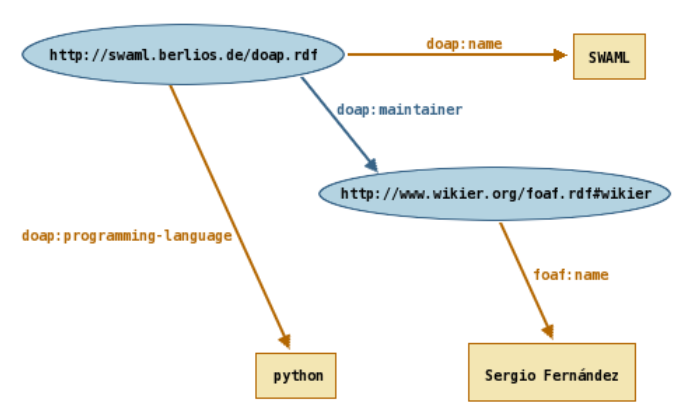
\includegraphics[width=0.8\textwidth]{images/grafo-rdf.png}
  \end{center}


}
\frame
{
  \frametitle{Ontología}

  \note[item] { Una ontología trata de describir o proponer las categorías y relaciones básicas. }
  \note[item] { En informática hace referencia al intento de formular un exhaustivo 
		y riguroso esquema conceptual dentro de un dominio dado. }
  \begin{columns}
   \begin{column}{0.55\textwidth}
	\begin{itemize}
	 \item Forma describir categorías y relaciones básicas.
	 \item Formulación un exhaustiva y rigurosa del esquema conceptual de un dominio dado.
	 \item OWL, lenguaje propuesto por el W3C para describir ontologías en la Web.
	 \item Varios ejemplos: FOAF, SIOC, Dublin Core, SKOS...
	\end{itemize}
   \end{column}
   \begin{column}{0.45\textwidth}
	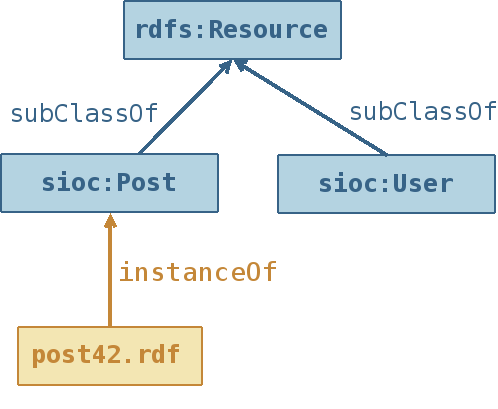
\includegraphics[width=0.9\textwidth]{images/ontologia.png}
   \end{column}
  \end{columns}




}

\section{El proyecto SWAML}

\subsection{Tecnologías implicadas}
\frame
{
  \frametitle{Tecnologías implicadas}

  \begin{itemize}
    \item<2-> \textbf{Python}: lenguaje de script orientado a objetos.
    \item<3-> \textbf{RDFLib}: biblioteca de Python para trabajar con RDF.
    \item<4-> \textbf{SIOC}: Semantically-Interlinked Online Communities.
  \end{itemize}

  \begin{center}
 	\only<2-3>{
\includegraphics[width=0.65\textwidth]{images/python.png}}
 	\only<4>{
\includegraphics[width=0.35\textwidth]{images/sioc.png}}
  \end{center}
}

\subsection{SWAML}
\frame
{
  \frametitle{SWAML}

  \begin{columns}
   \begin{column}{0.35\textwidth}
	El proyecto SWAML se compone de varias partes:
	\begin{itemize}
	 \item \begin{Large}SWAML\end{Large}
	 \item \begin{Large}Buxon\end{Large}
	 \item Herramientas complementarias
	\end{itemize}
   \end{column}
   \begin{column}{0.65\textwidth}
	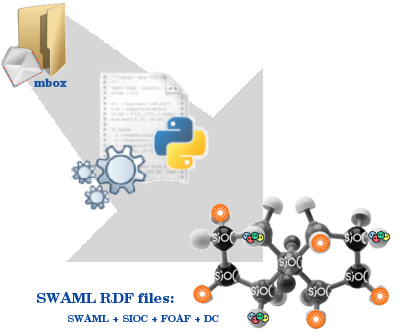
\includegraphics[width=0.95\textwidth]{images/swaml.png}
   \end{column}
  \end{columns}
}
\frame
{
  \frametitle{SWAML Core}

  \begin{columns}
   \begin{column}{0.5\textwidth}
	\begin{center}
	  \only<1>{
\includegraphics[width=0.95\textwidth]{images/swaml-0.png}}
	  \only<2>{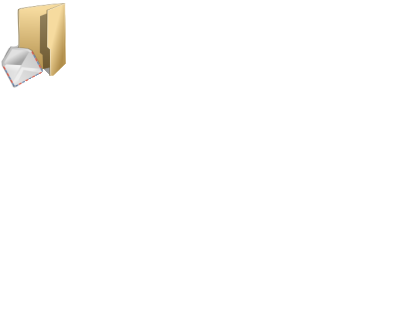
\includegraphics[width=0.95\textwidth]{images/swaml-1.png}}
	  \only<3>{
\includegraphics[width=0.95\textwidth]{images/swaml-2.png}}
	  \only<4>{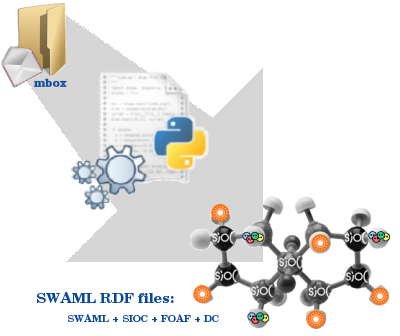
\includegraphics[width=0.95\textwidth]{images/swaml-3.png}}
	\end{center}
   \end{column}
   \begin{column}{0.5\textwidth}
	\begin{Large}Proceso batch:\end{Large}
	\begin{enumerate}
	 \item<2-> mbox
	 \item<3-> parsear
	 \item<4-> serializar a RDF/XML 
	\end{enumerate}
   \end{column}
  \end{columns}
}
\frame
{
  \frametitle{sioc:Forum}
  \begin{center}
    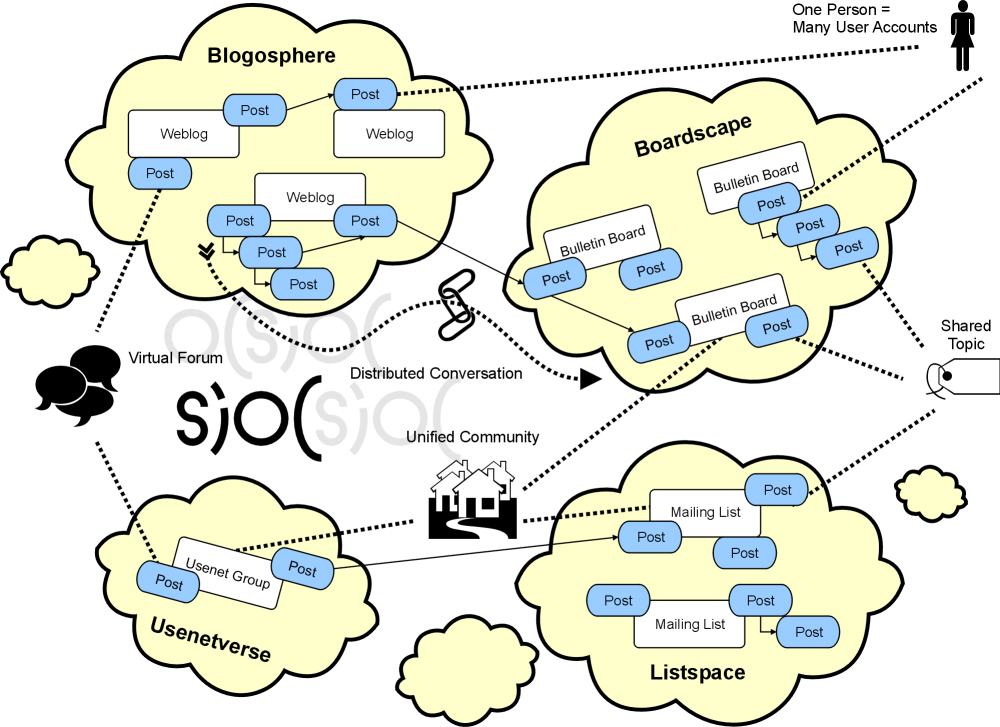
\includegraphics[width=0.8\textwidth]{images/sioc-discussions.png}
  \end{center}
}

\frame
{
  \frametitle{Buxon}

  \note[item] {	Desarrollado para demostrar que la representación en RDF de 
		una lista de correo permite volver recomponerla sin pérdida 
		de información. }
  \note[item] {	Implementación más madura para la explotación de datos SIOC. }

  \begin{columns}
   \begin{column}{0.32\textwidth}
	\begin{itemize}
	  \item Visor de \texttt{sioc:Forum}'s
	  \item Recomposición de la lista de correo
	  \item Implementación más completa de SIOC
	\end{itemize}
   \end{column}
   \begin{column}{0.68\textwidth}
	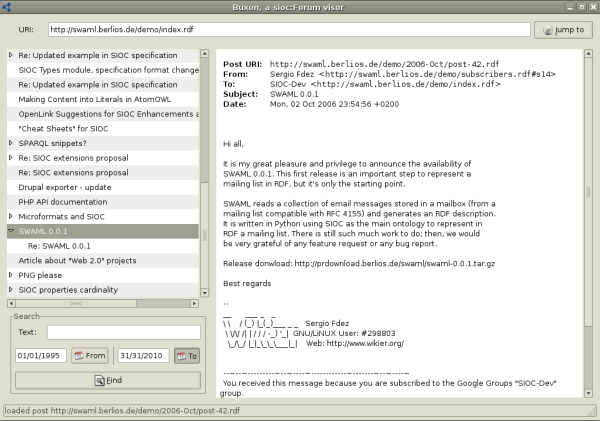
\includegraphics[width=\textwidth]{images/buxon.png}
   \end{column}
  \end{columns}
}
\frame
{
  \frametitle{Herramientas complementarias}

  \begin{itemize}
   \item<1-> \textbf{configWizard}: asistente de configuración mediante reflectividad estructural
   \item<2-> \textbf{FOAF Enricher}: enriquecedor de datos basado en FOAF
   \item<3-> \textbf{KML Exporter}: exportación de datos para Google Maps y Google Earth
  \end{itemize}

  \begin{center}
 	\only<2>{
\includegraphics[width=0.4\textwidth]{images/foaf.png}}
 	\only<3>{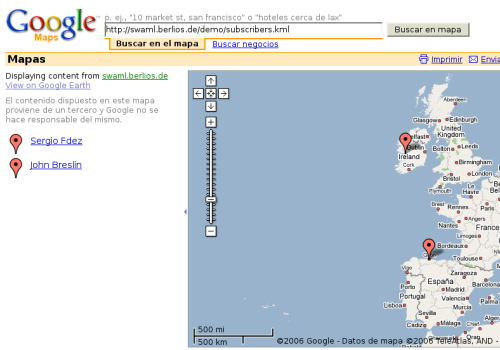
\includegraphics[width=0.55\textwidth]{images/googlemaps.png}}
  \end{center}

}

\section{Conclusiones}
\subsection{Impacto}
\frame
{
  \frametitle{Impacto}

  \begin{itemize}
   \item<1-> En palabras del propio John Breslin:
	\begin{quotation}
 	  El proyecto de SWAML satisface un requisito muy necesario para la Web semántica: 
	  poder referir a versiones semánticas de los mensajes de correo electrónico usando
	  un URI.
	\end{quotation}
   \item<2-> Aporta dos implementaciones a SIOC
   \item<3-> Acompaña a SIOC en el inminente proceso de \textit{submission} al W3C
  \end{itemize}

}
\subsection{Futuro}
\frame
{
  \frametitle{Futuro a medio plazo}
  \begin{itemize}
   \item \begin{Large}Acceder a cuentas de GMail\end{Large}
   \item \begin{Large}Marcado semántico para el cuerpo de los mensajes\end{Large}
   \item \begin{Large}API en Python para SIOC\end{Large}
   \item \begin{Large}Integración con Mailman\end{Large}
   \item \begin{Large}Paquete en Debian GNU/Linux\end{Large}
   \item \begin{Large}\textit{Submission} al W3C\end{Large}
  \end{itemize}
}

\section{Demostración}
\subsection{Demostración}
\frame
{
  \note[item]{Si no desean realizar ningún comentario, procederé a realizar una demostración práctica.}
  \note[item]{Ejemplo de exportación con SWAML (con todas las opciones), enseñar los RDF en plano.}
  \note[item]{Visualizarla con Buxon.}
  \note[item]{¿Algún ejemplo de SPARQL?}
  \note[item]{Terminar enseñando el KML en Google Maps}

  \begin{center}
    \LARGE{\textbf{demostración práctica}}
  \end{center}
}
\subsection{Preguntas}
\frame
{
  \note[item]{Agradecer la atención prestada.}
  \note[item]{Quedar a disposición del tribunal para contestar a las
		preguntas o ampliar cualquiera de los temas expuestos.}

  \begin{center}
    \LARGE{\textbf{SWAML, publicación de listas de correo en web semántica}}\\
    \vspace{1cm}
    \LARGE{Fin}\\
    \vspace{2cm}
    \begin{tiny}
	Esta presentación se distribuye bajo los términos de la licencia
	CreativeCommons Reconocimiento-CompartirIgual 2.5
    \end{tiny}
  \end{center}
}

\appendix

\section{Respuestas preparadas}
\frame{
  FIXME: SPARQL, UML, etc
}


\end{document}
